\chapter{Implementation}
\label{sec:implementation}

% Hier greift man einige wenige, interessante Gesichtspunkte der
% Implementierung heraus. Das Kapitel darf nicht mit Dokumentation oder
% gar Programmkommentaren verwechselt werden. Es kann vorkommen, daß
% sehr viele Gesichtspunkte aufgegriffen werden müssen, ist aber nicht
% sehr häufig. Zweck dieses Kapitels ist einerseits, glaubhaft zu
% machen, daß man es bei der Arbeit nicht mit einem "Papiertiger"
% sondern einem real existierenden System zu tun hat. Es ist sicherlich
% auch ein sehr wichtiger Text für jemanden, der die Arbeit später
% fortsetzt. Der dritte Gesichtspunkt dabei ist, einem Leser einen etwas
% tieferen Einblick in die Technik zu geben, mit der man sich hier
% beschäftigt. Schöne Bespiele sind "War Stories", also Dinge mit denen
% man besonders zu kämpfen hatte, oder eine konkrete, beispielhafte
% Verfeinerung einer der in Kapitel 3 vorgestellten Ideen. Auch hier
% gilt, mehr als 20 Seiten liest keiner, aber das ist hierbei nicht so
% schlimm, weil man die Lektüre ja einfach abbrechen kann, ohne den
% Faden zu verlieren. Vollständige Quellprogramme haben in einer Arbeit
% nichts zu suchen, auch nicht im Anhang, sondern gehören auf Rechner,
% auf denen man sie sich ansehen kann.

\begin{itemize}

\item The CAL with Policy Based Design

  In section \ref{sec:cal} the CAL was introduced as an flexible
  Communication layer based on varying adapters. For the implementation
  of the varying adapters, a policy based design was choosen.

  A policy is a class or or class template interface, which consists of
  inner type definitions, member functions and or member variables. An
  implementation of a policy is called policy class and is inherited
  by or contained within a host class.

  The advantage of policy based design is that the variable
  functionality of the policy is bounded to its host class at compile
  time, providing no runtime overhead. And the interface of the policy
  is strictly defined by the host class. Ignoring this interface leads
  to errors at compile time.

  This means, that an adapter is a policy, here called communication
  policy, and the CAL is the host class (Figure \ref{fig:cal_uml}).

  \begin{figure}[H]
    \centering 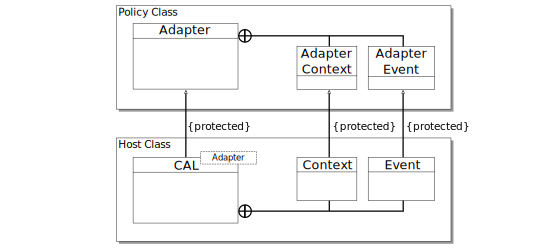
\includegraphics[width=\textwidth]{graphics/40_cal_uml}
    \caption{  }
    \label{fig:cal_uml}
  \end{figure}



  The CAL defines the interface for context , peer to peer
  and collective functions. The Adapter has to implement the
  functionality of these functions.



  The CAL defines the policy class interfaces as follows:

  \begin{itemize}
    \item Type Definitions
      \begin{itemize}
      \item Context 
      \item Event
      \item Virtual Address
      \end{itemize}

    \item Member Functions
      \begin{itemize}
      \item asyncSendData
      \item asyncRecvData

      \item gather
      \item gather2
      \item allGather
      \item allGather2
      \item scatter
      \item allToAll
      \item reduce
      \item allReduce
      \item broadcast
      \item synchronize

      \item getGlobalContext
      \item createContext
      \end{itemize}
     

  \item Member Variables
      \begin{itemize}
        \item 
      \end{itemize}

  \end{itemize}


  \begin{itemize}
  \item Communication Policy forms Adapters
  \item Requirements to the Communication Policy
  \item The MPI Adapter
    \begin{itemize}
    \item Abitrary Binary Operation
    \item Builtin Type Conversion 
    \end{itemize}
  \item Context
  \item Event
  \end{itemize}

\item Graph Based on the Boost Graph Library
  \begin{itemize}
  \item Vertices identified by Properties
  \item Creation of subgraphs
  \end{itemize}
  
\item Configuration of an Application by Templates
  \begin{itemize}
  \item Creation of a Graph
  \item Example Configuration of a Communication System
  \end{itemize}

\item Implementing a Game of Life
  \begin{itemize}
  \item Based on Cells
  \item Based on Bundles
  \end{itemize}

\end{itemize}




\cleardoublepage

%%% Local Variables:
%%% TeX-master: "diplom"
%%% End:
